%!TEX program = xelatex
% 完整编译方法 1 pdflatex -> bibtex -> pdflatex -> pdflatex
% 完整编译方法 2: xelatex -> bibtex -> xelatex -> xelatex
\documentclass[lang=cn,11pt]{elegantpaper}
\usepackage{url}
\usepackage{booktabs}
\usepackage{multirow}
\usepackage{geometry}
\usepackage{longtable}
\usepackage{pdfpages}
\title{集成学习的一次实践}

% 不需要版本信息, 直接注释即可
% \version{0.07}
% 不需要时间信息的话, 需要把 \today 删除. 
\date{}


% 如果想修改参考文献样式, 请把这行注释掉
% \usepackage[authoryear]{gbt7714}  % 国标

\begin{document}


\newpage
\maketitle

	
\tableofcontents
\thispagestyle{empty}
\newpage
\normalsize
\pagenumbering{arabic}


\section{前言}

集成学习是指使用多种兼容的学习算法或模型来执行单个任务的技术, 目的是为了得到更佳的预测表现. 集成学习的主要方法可归类为三大类: 堆叠(Stacking)、提升(Boosting)和装袋. 其中最流行的方法包括随机森林、梯度提升、AdaBoost、梯度提升决策树(GBDT)和XGBoost. 

1979年, Dasarathy 提出集成系统(ensemble system)的思想, 并使用线性分类器和最近邻居(NN)分类器组成的复合系统作为其组成部分的例子来说明这些概念. 1988年Kearns和1989年Valiant分别提出的弱学习的概念, 引发了关于“能否用一组弱学习器创造一个强学习器”这一问题的讨论. 1990年Schapire对这一问题给出了肯定的回答, 并开发出boosting. 并在几年之后和Freund提出了AdaBoost, 该算法被广泛使用, 他们还凭借Adaboost获得了计算机领域富有盛名的哥德尔奖. 1996年, Breiman 开发出 Bagging 预测器, 并对其原理和训练进行了详细描述. 

近年来, boosting算法在数据科学或机器学习竞赛中得到了广泛的普及, 这些比赛的大多数获胜者都使用boosting算法来实现高精度. 这些数据科学竞赛为学习、探索和为各种商业和政府问题的解决方案提供了全球性的平台. Boosting算法结合了多个低精度模型来创建一个高精度模型. 它可以用于各种领域, 例如信贷、保险、市场营销和销售. 

\section{集成学习介绍}

集成是一个组合模型, 它结合了一系列性能低下的分类器, 目的是创建一个性能更好的分类器. 集成的方法提供比单个或基本分类器更高的准确性, 也可以说集成学习方法是将几种机器学习方法组合到单个预测模型中以提高性能的元算法. 集成方法可以使用bagging方法减少方差, 使用boosting方法减少偏差, 或者使用stacking方法来改善预测. 
\begin{figure}[htbp]
  \centering
  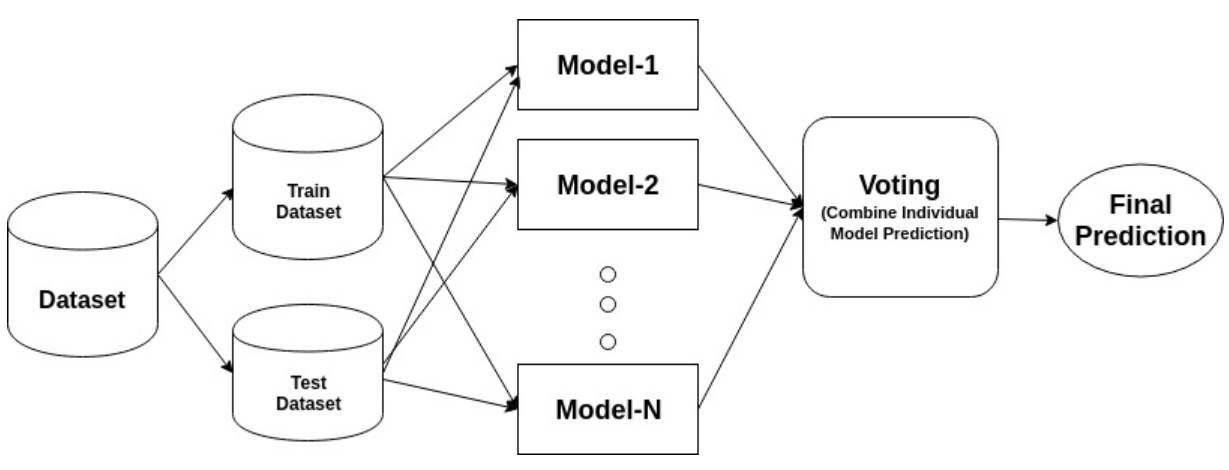
\includegraphics[width=0.7\textwidth]{1}
  \caption{三种机器学习方法.}
\end{figure}
\subsection{集成学习的方法}
一般在集成学习中, 我们会用到三种方法. 
\subsubsection*{Bagging算法}
Bagging算法代表着引导聚集(Bootstrap aggregating), 它为了减少估计的方差组合了多个学习机. 例如, 随机森林训练了M个决策树, 那便可以在数据的不同随机子集上训练M个不同的树, 并对最终预测进行投票. Bagging算法也可与其他分类、回归算法结合, 提高其准确率、稳定性的同时, 通过降低结果的方差, 避免过拟合的发生. 
\subsubsection*{Boosting算法}
Boosting算法是一种能够将弱学习器转化为强学习器, 从而提升各种学习算法的方法. 理论上, boosting 可以显著减小弱学习器的偏差, 这些弱学习器的效果只是稍微优于随机猜测, 比如小决策树——数据加权模型. 然后Boosting在运行时将更多的权重赋值给早期训练中错误最多的数据集, 通过结合加权多数投票(分类)或加权求和(回归)以产生最终预测. Boosting的每个模型都是单独运行, 每个模型决定下一个模型要关注的特征, 最后在不偏向任何模型的前提下聚合输出结果. 
\subsubsection*{Stacking算法}
Stacking算法是一种集成学习技术, 用于最小化一个或多个泛化器的泛化误差率的方法. 它通过推导泛化器相对于所提供的学习集的偏差来发挥其作用. 这个推导的过程包括:在第二层中将第一层的原始泛化器对部分学习集的猜测进行泛化, 以及尝试对学习集的剩余部分进行猜测, 并且输出正确的结果. 当与多个泛化器一起使用时, 堆叠泛化可以被看作是一个交叉验证的复杂版本, 利用比交叉验证更为复杂的策略来组合各个泛化器. 当与单个泛化器一起使用时, 堆叠泛化是一种用于估计(然后纠正)泛化器的错误的方法, 该泛化器已经在特定学习集上进行了训练并被询问了特定问题. 
\begin{figure}[htbp]
  \centering
  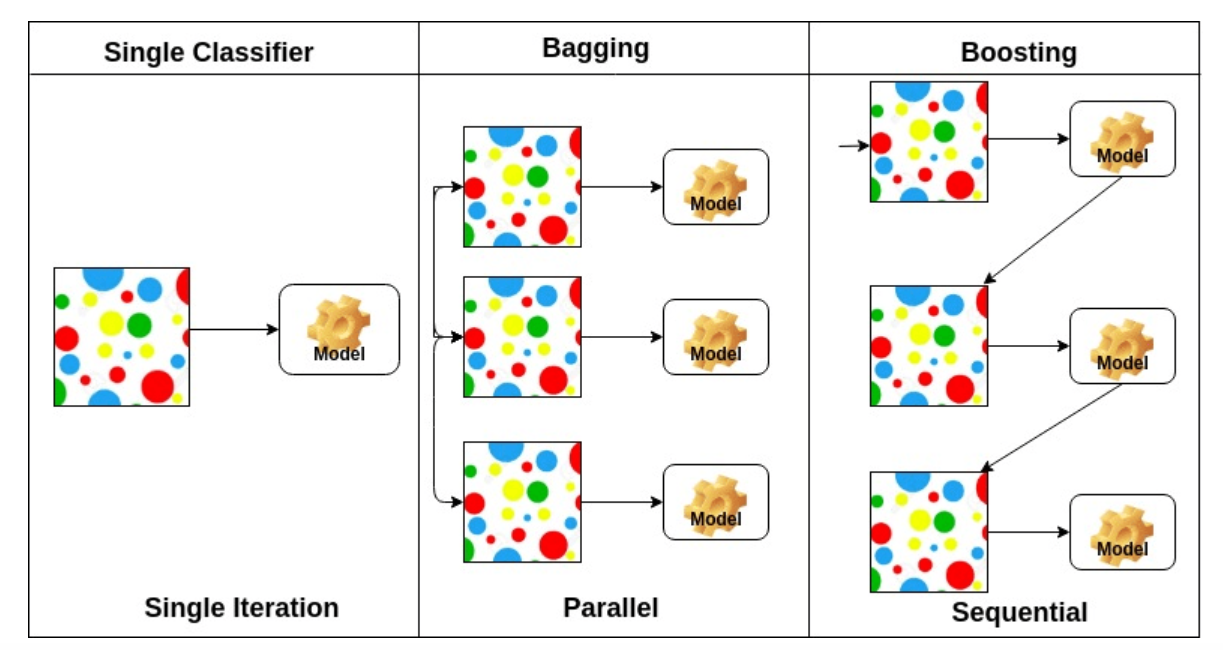
\includegraphics[width=0.7\textwidth]{2}
  \caption{基于Stacking算法的分类.}
\end{figure}

以基学习器的分布为基础, stacking方法可以分为两组:在平行集成方法中, 基学习器平行的产生, 例如随机森林. 在顺序集成方法中, 基学习器是顺序生成的, 例如AdaBoost;

以基学习器的类型也可以分为两组:同构集成方法在每次迭代中使用相同类型的基学习器. 异构集成方法在每次迭代中使用不同类型的基学习器. 
\section{模型介绍}
AdaBoost是一种迭代集成方法. AdaBoost分类器通过组合多个性能不佳的分类器来构建一个强分类器. AdaBoost背后的基本概念是设置分类器的权重, 并在每次迭代中训练数据样本, 从而确保对异常观测值的准确预测. 任何机器学习算法在接受了训练集上的权重后, 都可以被当作基学习器. AdaBoost应该满足两个条件:
\begin{enumerate}
  \item 分类器应在各种加权的训练示例上进行交互训练. 
  \item 在每次迭代中, 它都试图通过最小化训练误差为这些示例提供出色的拟合. 
\end{enumerate}
\subsection{AdaBoost步骤}
\begin{figure}[htbp]
  \centering
  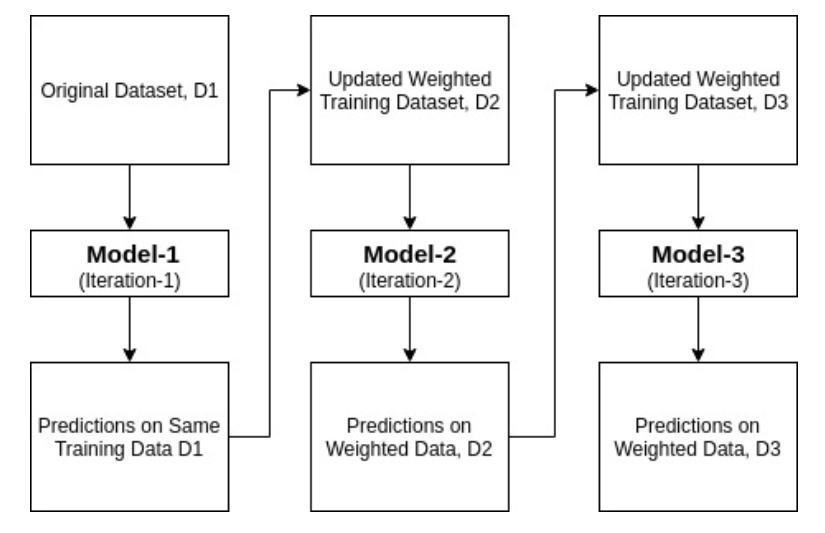
\includegraphics[width=0.7\textwidth]{3}
  \caption{AdaBoost步骤示意图.}
\end{figure}
\begin{enumerate}
  \item Adaboost先随机选择一个训练子集. 
  \item 基于上次训练的准确预测来选择训练集来迭代训练AdaBoost模型. 
  \item 将较高的权重分配给错误的分类观测值, 以便在下一次迭代中这些观测值将获得较高的被分类概率. 
  \item 根据分类器的准确性在每次迭代中将权重分配给经过训练的分类器. 分类器越准确, 权重越高. 
  \item 反复进行此过程, 直到完整的训练数据正确无误或达到指定的最大估计量为止. 
  \item 最后, 让所有构建的所有学习算法进行“投票”, 获取分类结果.   
\end{enumerate}
\subsection{模型训练}
我们使用了sklearn中ensemble类里的AdaBoostClassifier类. 数据集选用了UCI数据集中的IRIS数据集. IRIS数据集是一个花卉分类数据集, 其中给出了标记好的三种花卉(Iris Setosa-山鸢尾, Iris Versicolour-杂色鸢尾, 以及Iris Virginica-维吉尼亚鸢尾, 每类包含50个样本), 以及其所对应的四个特征(花萼长度, 花萼宽度, 花瓣长度, 花瓣宽度). 我们的任务是学习一个函数, 使得其通过输入这三种花其中的某一种的一个植株的这四个参数, 能够判断出这个植株是哪一种花. 这是一个典型的分类问题, IRIS数据集也是应用广泛的数据分类数据集. 我们首先将数据集分为训练集与测试集两部分进行训练.

\begin{figure}[htbp]
\centering
  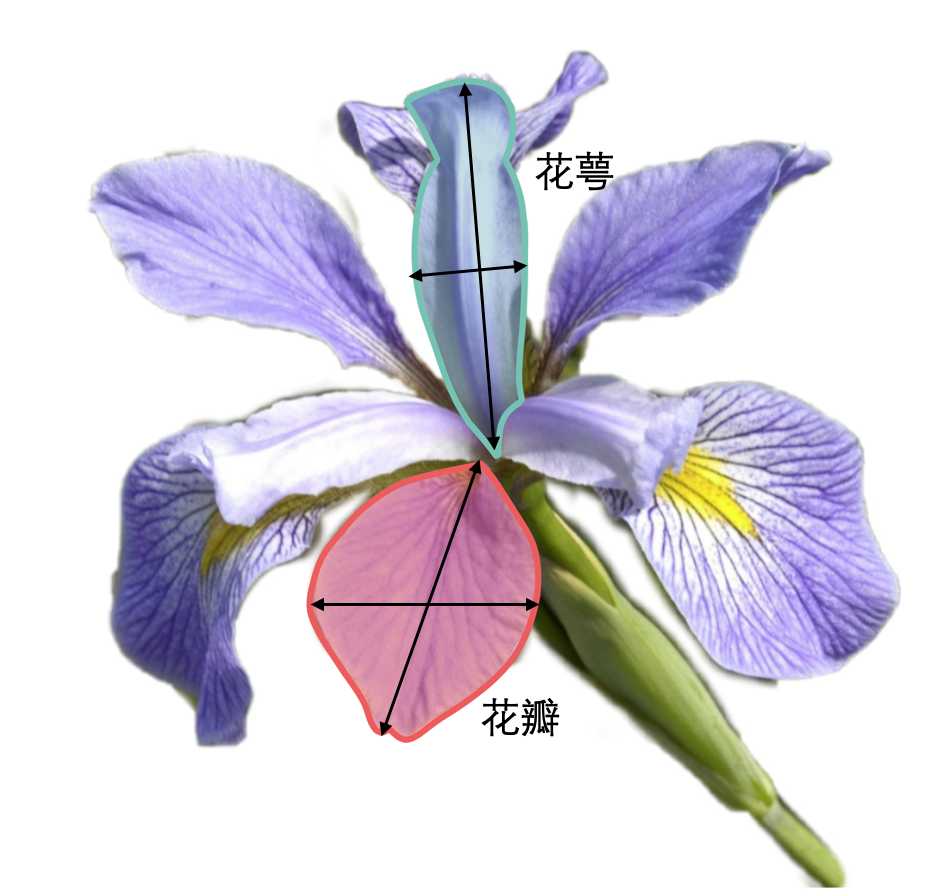
\includegraphics[width=0.2\textwidth]{flower.png}
  \caption{弗吉尼亚莺尾的花萼与花瓣示意图\label{fig:VGflower}}
\end{figure}


\subsection{决策树弱学习机}

我们的模型采用了50个决策树作为弱学习机, 采用了默认的学习率1. Sklearn的AdaboostClassifier能够全自动地帮我们完成优化损失函数%\todo{损失函数是啥}. 
我们在测试集上获得了
的准确率. 


我们还尝试可视化了我们模型的分类边界. 不过由于四维的数据可视化起来比较困难. 我们右只在其中的两个特征上使用相同的方法与参数训练出来了一个学习机, 虽然在性能上有着不小的损失, 准确率从掉到了

, 不过我们觉得很好地解释了我们习得的分类器. 从图上也可以看出这两个特征可以很好的将A类与B、C类分开, 但是对于B、C类之间的分类做的很差. 除了这两个特征我们需要更多的信息去区分B、C类. 

--------------!!!!!BC是哪两类, 特征你用的啥?? 第二个图你解释一下


\subsection{学习机数量提升}

%\todo{改个参数}

那么一个最简单的改进的思路就是去增加弱学习机的数量, 通过更大的学习规模去对函数做更好的拟合. 




我们采用了相同的可视化方案, 重新构建了一个学习机利用两个特征进行分类. 我们的得到的可视化结果与上一次基本上相同, 边的位置有了调整. 意味着增大我们的学习规模虽然可以在一定程度上提升我们分类的准确性, 找到更好的分类边界, 但是其并没有改变分类边界是直线这一致命缺陷, 导致了我们的分类结果的提升非常有限.

\subsection{支撑向量机弱学习机}

由于Boosting过程的特性, 另外一个显然的想法就是尝试不同的弱学习机去提升我们的分类准确率. 我们又尝试了支撑向量机作为我们的弱学习机去进行Adaboosting学习. sklearn.svm类中的svc类给我们提供这样现成的弱学习机. 在支撑向量机里, 我们采用了线性的核函数. 通过使用相同的参数, 我们发现这样的弱学习机的选取也可以极大程度上的影响我们的分类准确率. 我们的分类准确率从%\todo{提升}

提升到了

依旧我们对于两个特征又训练了一个模型用于可视化, 其准确率从

并且可以从图上观察出我们的分类器的确能够相比采用决策树时更好地捕捉到类边界. 相比于决策树的边界而言, SVM作为弱学习机习得的边界不再是一条直线, 故显著增加了分类准确性. 我们还可以观察到在A类与B、C类的分离时几乎没有错分, 但是我们依旧需要更多的信息去区分B、C类.



\newpage
\nocite{*}

% 如果想修改参考文献样式( 非国标 ), 请把下行取消注释, 并换成合适的样式( 比如 unsrt, plain 样式 ). 
\bibliographystyle{unsrt}
\bibliography{wpref}

\end{document}
